\chapter{États, mesures et espaces vectoriels complexes}

\lectureoverview{La mécanique quantique commence par changer notre conception de l’état. Nous isolons d’abord le schéma classique des états et de leur évolution déterministe, puis nous en mettons en évidence les limites à l’aide d’une expérience de spin à deux issues. La réponse mathématique est un espace vectoriel complexe muni de vecteurs duaux, d’un produit scalaire, d’une norme et d’une notion d’orthogonalité.}

\section{Le schéma classique : état et évolution}

Commençons par un système fermé, au moins provisoirement isolé de tout le reste. Ici, le mot \emph{système} est un terme primitif : il désigne l’objet dont nous voulons prédire l’histoire. Un \emph{état} comprend tout ce qu’il faut connaître à un instant donné pour effectuer cette prédiction. La mécanique classique fournit une loi qui fait évoluer un état vers le suivant.

Pour une pièce abstraite des plus simples,
\begin{equation}
  \mathcal S_{\mathrm{coin}}=\{H,T\}.
\end{equation}
Une loi possible stipule que rien ne se passe :
\begin{equation}
  H\longmapsto H,
  \qquad
  T\longmapsto T.
\end{equation}
Une autre loi alterne les deux états :
\begin{equation}
  H\longmapsto T,
  \qquad
  T\longmapsto H.
\end{equation}
Ces exemples sont élémentaires, mais ils mettent en évidence l’architecture d’une théorie classique :
\begin{equation}
  s(t)\longmapsto s(t+\Delta t).
\end{equation}
Une fois que \(s(t)\) est connu, l’évolution est déterministe.

Le même schéma vaut lorsque l’espace des états est continu. Une particule se déplaçant sur une droite requiert à la fois sa position et sa quantité de mouvement,
\begin{equation}
  s=(q,p),
\end{equation}
son espace des états est donc le plan des phases. Le nombre d’états possibles est devenu infini et les équations peuvent s’écrire dans le langage élégant des lagrangiens, des hamiltoniens et des crochets de Poisson, mais l’idée sous-jacente n’a pas changé. L’état à un instant donné contient ce qu’il faut pour prédire l’état à un autre instant.

\section{L’abstraction avant la visualisation}

Le mouvement classique est relativement facile à se représenter, car ses concepts sont tirés de l’expérience ordinaire. Cet avantage disparaît lorsque les objets concernés sont trop petits, que les vitesses sont trop grandes ou que l’espace des états comporte trop de dimensions. Personne ne se représente littéralement le mouvement d’un électron, l’espace-temps à quatre dimensions ou un espace à dix dimensions. Ce n’est pas une difficulté propre aux débutants. L’intuition visuelle humaine s’est formée dans le monde quotidien à trois dimensions.

Même des cas apparemment plus simples révèlent cette limite. Ce que nous appelons l’image d’un espace courbe à deux dimensions est ordinairement une surface plongée dans un espace à trois dimensions. Une droite à une dimension se représente comme un trait dans un plan. L’image fait discrètement intervenir l’espace ambiant dans lequel notre système visuel sait fonctionner.

La solution ne consiste pas à imposer une image classique à une physique qui nous est étrangère. Il s’agit d’apprendre la structure abstraite et de laisser une nouvelle intuition se développer à partir de manipulations correctes. Les coordonnées tridimensionnelles \((x,y,z)\) deviennent des coordonnées à quatre dimensions \((x,y,z,w)\) par l’ajout d’un symbole et l’extension des règles, et non par l’acquisition d’un nouvel organe de la vue. La mécanique quantique exige la même discipline. La traiter comme un modèle mécanique étrange composé de petits objets classiques conduit sans cesse à de mauvaises réponses.

\begin{remark}
L’intuition mathématique se développe tout de même. Elle n’est simplement pas la même que celle qui consiste à voir une vague sur l’océan ou une flèche dans l’espace ordinaire. L’algèbre devient familière parce que ses relations sont utilisées de façon cohérente.
\end{remark}

\section{Espaces des états classiques et logique classique}

Pour un système classique, l’espace des états est un ensemble. Un dé abstrait possède
\begin{equation}
  \mathcal S_{\mathrm{die}}=\{1,2,3,4,5,6\}.
\end{equation}
Un dé réel peut prendre une infinité continue d’orientations, mais le dé idéalisé utilisé ici ne possède que ces six étiquettes. Une particule sur une droite possède l’ensemble infini continu
\begin{equation}
  \mathcal S_{\mathrm{particle}}
  =
  \{(q,p)\mid q,p\in\mathbb R\}.
\end{equation}
Qu’il soit fini ou infini, tout espace des états classique est un ensemble de possibilités mutuellement distinctes.

Une proposition concernant le système sélectionne un sous-ensemble de ces possibilités. Pour le dé, posons
\begin{align}
  P_{\mathrm{odd}}&=\{1,3,5\},\\
  P_{\leq 3}&=\{1,2,3\}.
\end{align}
L’énoncé \emph{impair et inférieur ou égal à trois} correspond à leur intersection :
\begin{equation}
  P_{\mathrm{odd}}\cap P_{\leq 3}=\{1,3\}.
\end{equation}
L’énoncé inclusif \emph{impair ou inférieur ou égal à trois} correspond à leur réunion :
\begin{equation}
  P_{\mathrm{odd}}\cup P_{\leq 3}
  =
  \{1,2,3,5\}.
\end{equation}
La conjonction et la disjonction classiques prennent donc la forme ensembliste suivante :
\begin{equation}
  P\wedge Q\longleftrightarrow P\cap Q,
  \qquad
  P\vee Q\longleftrightarrow P\cup Q.
\end{equation}
Si les sous-ensembles ne se recoupent pas, aucun état ne rend les deux propositions vraies.

Cette logique est liée à la conception classique de l’état. La mécanique quantique remplace l’ensemble des alternatives classiques par un autre objet mathématique : un espace vectoriel. Ce n’est que dans une limite classique appropriée que la description par un espace vectoriel se comporte approximativement comme un ensemble de configurations exclusives. Avant de construire cet espace, il nous faut une expérience qui rende ce remplacement incontournable.

\section{Le système quantique le plus simple}

L’analogue quantique de la pièce abstraite est un système à deux issues appelé \emph{qubit}. On peut d’abord désigner ses issues mesurées par pile et face, mais une étiquette numérique est plus utile :
\begin{equation}
  \sigma\in\{+1,-1\}.
\end{equation}
Trois notations seront utilisées en parallèle :
\begin{equation}
  H\longleftrightarrow \sigma=+1\longleftrightarrow\uparrow,
  \qquad
  T\longleftrightarrow \sigma=-1\longleftrightarrow\downarrow.
\end{equation}
Au départ, les flèches ne sont que des noms. On n’a pas encore supposé qu’il s’agissait de vecteurs géométriques ordinaires.

\begin{figure}[htbp]
  \centering
  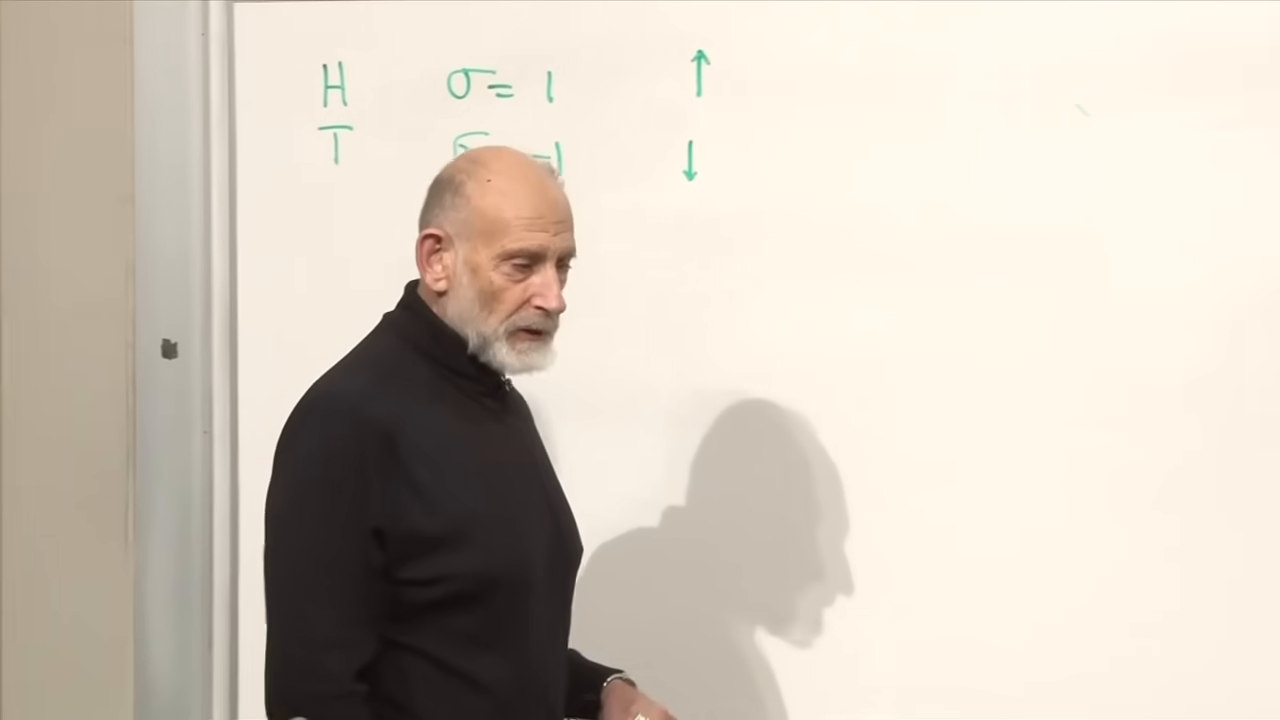
\includegraphics[width=0.78\textwidth]{lecture_01_figure_02.png}
  \caption{Le tableau présente les étiquettes équivalentes \(H/T\), \(\sigma=\pm1\) et les flèches haut/bas. Au départ, les flèches sont une notation, et non un modèle classique.}
  \lectureframe{00:22:44}
\end{figure}

\begin{classroomqa}
\audiencequestion{Quel rapport y a-t-il entre pile et face et le système physique ?}
\lecturerresponse{Rien d’autre que le fait de fournir deux noms familiers. Pour cette mesure, le qubit a deux issues possibles ; pile et face ne sont que des étiquettes provisoires. Les étiquettes \(\pm1\) sont choisies parce qu’elles peuvent figurer dans des équations.}
\end{classroomqa}

\subsection{L’appareil comme boîte noire}

Une expérience nécessite un second système, l’appareil \(A\). Pour l’instant, c’est une boîte noire abstraite dotée de trois caractéristiques :
\begin{enumerate}
  \item il a une orientation spatiale, indiquée par \emph{ce côté vers le haut} ;
  \item il a un capteur qui peut interagir avec le qubit ;
  \item il a un affichage initialement vierge, qui indique ensuite \(+1\) ou \(-1\).
\end{enumerate}
Les détails du détecteur sont délibérément laissés de côté pour le moment. Un bon détecteur se définit de façon opérationnelle par la relation fiable entre le système et l’enregistrement qu’il fournit. L’observateur n’a pas besoin d’assister à l’interaction : l’appareil peut enregistrer le résultat, qui sera lu plus tard.

Supposons que l’affichage indique \(+1\). Remettons l’appareil à zéro, dans son état vierge, puis répétons immédiatement la même mesure, avant que la moindre évolution indépendante ait le temps d’agir. Un détecteur fidèle indique de nouveau \(+1\). Si le premier résultat est \(-1\), les répétitions immédiates continuent de même à indiquer \(-1\) :
\begin{equation}
\begin{aligned}
  +1&\longrightarrow +1\longrightarrow +1\longrightarrow\cdots,\\
  -1&\longrightarrow -1\longrightarrow -1\longrightarrow\cdots.
\end{aligned}
\end{equation}
On peut donc considérer la première mesure comme une \emph{préparation}. Elle laisse le qubit dans un état où une répétition immédiate de la même mesure donne un résultat déterminé.

Cette répétabilité n’est pas une simple interprétation philosophique facultative. Sans elle, il n’existerait aucun moyen opérationnel de confirmer une mesure. Un appareil défectueux peut ne pas reproduire son résultat, mais il n’effectue alors pas la mesure idéale que nous sommes en train de définir.

\begin{classroomqa}
\audiencequestion{S’agit-il déjà de l’effondrement de la fonction d’onde ?}
\lecturerresponse{Nous pourrons introduire ce vocabulaire plus tard. À ce stade, l’énoncé opérationnel suffit : une mesure produit un résultat et prépare un état dans lequel la même mesure, répétée immédiatement, reproduit ce résultat. Donner un nom au processus ne l’explique pas encore.}
\end{classroomqa}

\section{Orientation et échec de l’aiguille classique}

Préparons le qubit de sorte que l’appareil en position verticale indique \(+1\). Faisons tourner l’appareil de \(180^\circ\) et répétons la mesure. Le résultat est alors \(-1\). Des mesures répétées avec l’appareil inversé confirment \(-1\), tandis que le remettre en position verticale rétablit \(+1\).

Le résultat révèle une véritable dépendance à la direction. La notation haut/bas n’est pas entièrement arbitraire : inverser le détecteur inverse le signe. On pourrait être tenté d’en conclure que le qubit est simplement un petit vecteur et que le détecteur mesure la composante de ce vecteur selon son propre axe. Il faut mettre cette idée à l’épreuve plutôt que s’y fier.

\begin{figure}[htbp]
  \centering
  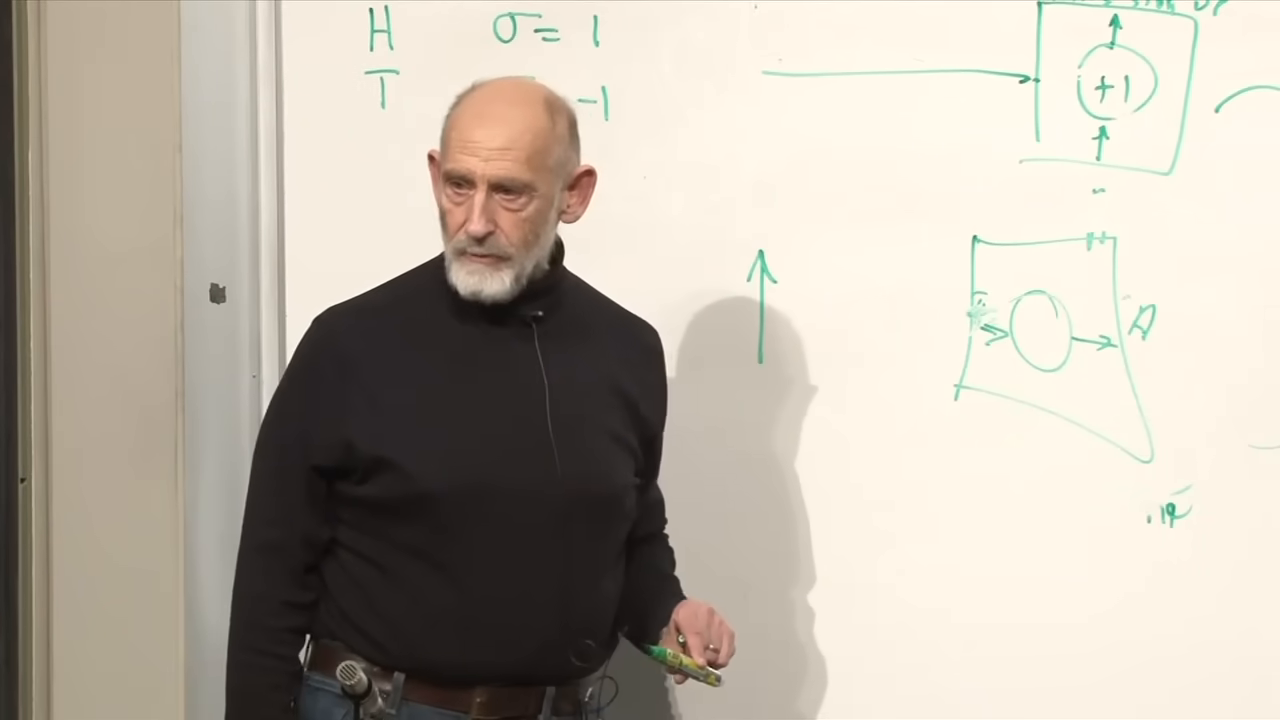
\includegraphics[width=0.82\textwidth]{lecture_01_figure_03.png}
  \caption{Préparation vers le haut et analyseurs d’orientations différentes au tableau. La classe a ensuite corrigé le sens d’une flèche tracée à la craie ; seul l’axe de l’analyseur importe dans le raisonnement.}
  \lectureframe{00:36:21}
\end{figure}

\subsection{Une mesure latérale}

Tournons le détecteur de \(90^\circ\). Si le qubit préparé était une aiguille ordinaire orientée vers le haut, sa composante selon l’axe horizontal du détecteur serait nulle :
\begin{equation}
  \hat{\mathbf x}\cdot\hat{\mathbf z}=0.
\end{equation}
L’appareil quantique n’indique jamais zéro. Chaque essai donne soit \(+1\), soit \(-1\).

\begin{figure}[htbp]
  \centering
  \resizebox{\linewidth}{!}{%
  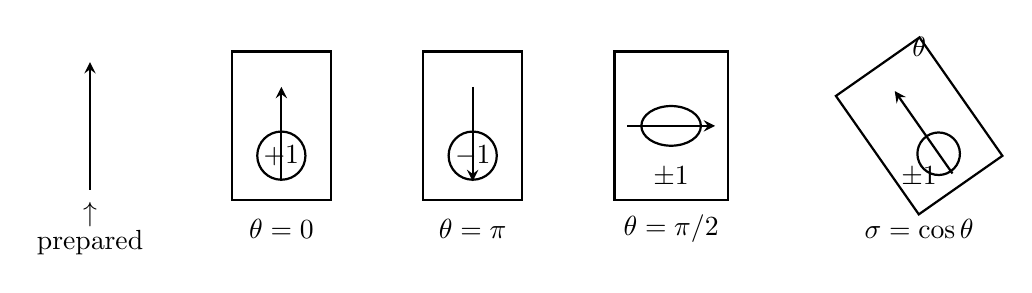
\begin{tikzpicture}[>=stealth,thick,scale=0.90]
    \draw[->] (0,0)--(0,1.8);
    \node at (0,-0.35) {\(\uparrow\)};
    \node at (0,-0.75) {prepared};

    \draw (2.0,-0.15) rectangle (3.4,1.95);
    \draw (2.7,0.48) circle (0.34);
    \draw[->] (2.7,0.12)--(2.7,1.45);
    \node at (2.7,0.48) {\(+1\)};
    \node at (2.7,-0.55) {\(\theta=0\)};

    \draw (4.7,-0.15) rectangle (6.1,1.95);
    \draw (5.4,0.48) circle (0.34);
    \draw[->] (5.4,1.45)--(5.4,0.12);
    \node at (5.4,0.48) {\(-1\)};
    \node at (5.4,-0.55) {\(\theta=\pi\)};

    \draw (7.4,-0.15) rectangle (9.0,1.95);
    \draw (8.2,0.90) ellipse (0.42 and 0.28);
    \draw[->] (7.58,0.90)--(8.82,0.90);
    \node at (8.2,0.18) {\(\pm1\)};
    \node at (8.2,-0.55) {\(\theta=\pi/2\)};

    \begin{scope}[shift={(11.7,0.90)},rotate=35]
      \draw (-0.72,-1.02) rectangle (0.72,1.02);
      \draw (0,-0.48) circle (0.30);
      \draw[->] (0,-0.82)--(0,0.60);
    \end{scope}
    \node at (11.7,0.18) {\(\pm1\)};
    \node at (11.7,-0.55) {\(\expect{\sigma}=\cos\theta\)};
    \node at (11.7,2.02) {\(\theta\)};
  \end{tikzpicture}
  }%
  \caption{Reconstitution de la séquence des analyseurs. Une rotation modifie les statistiques, jamais l’ensemble des issues individuelles.}
\end{figure}

Préparons un grand ensemble de qubits avec l’appareil en position verticale et conservons ceux pour lesquels le résultat est \(+1\). Mesurons chaque qubit conservé une fois avec l’appareil en position latérale. La moitié des essais donne \(+1\), l’autre moitié \(-1\), et la moyenne d’ensemble est nulle :
\begin{equation}
  \expect{\sigma}_{\pi/2}=0.
\end{equation}
La moyenne ressemble à la composante horizontale nulle d’une aiguille classique, mais les résultats individuels, eux, n’y ressemblent pas. La valeur classique \(0\) a été remplacée par un équilibre statistique entre deux issues discrètes.

\begin{classroomqa}
\audiencequestion{Que se passe-t-il si l’on garde le même qubit au lieu de l’écarter après la mesure latérale ?}
\lecturerresponse{Supposons que le premier résultat latéral soit \(+1\). Si l’on répète la mesure latérale sur ce même qubit, on obtient encore et encore \(+1\). La première mesure latérale l’a préparé par rapport à l’axe latéral. Pour obtenir des statistiques moitié-moitié, il faut répéter l’expérience complète de préparation et de mesure sur de nombreux qubits, et non confirmer plusieurs fois le même résultat.}
\end{classroomqa}

\subsection{Préparations incompatibles}

L’ordre des axes compte. Préparons le qubit avec \(+1\), puis effectuons une mesure horizontale. Le premier résultat horizontal est aléatoire. Une fois ce résultat obtenu, les répétitions immédiates de la mesure horizontale donnent un résultat déterminé. Revenons ensuite à l’axe vertical avec le détecteur. Le résultat vertical est de nouveau aléatoire.

En notant \(M_z\) et \(M_x\) les mesures selon les deux axes,
\begin{equation}
\begin{aligned}
  M_z&:+1,\\
  M_x&:\pm1,\\
  M_x&:\text{same result},\\
  M_z&:\pm1.
\end{aligned}
\end{equation}
la mesure intermédiaire selon \(x\) n’a pas simplement révélé une composante horizontale tout en préservant l’état vertical initial. Elle a préparé un nouvel état, et la certitude initiale concernant l’axe vertical a disparu.

\begin{classroomqa}
\audiencequestion{Le détecteur se souvient-il de la première réponse ? Comment peut-il savoir si on lui présente le même qubit ou un nouveau qubit ?}
\lecturerresponse{La répétabilité est une propriété du qubit mesuré ; elle ne résulte pas d’une comparaison avec une mémoire cachée dans le détecteur. Après une mesure, le qubit se trouve dans un état qui donne la même réponse à la même mesure immédiate. Si l’on présente un qubit préparé différemment, le résultat dépend de cette préparation. Suivre quel système physique est mesuré relève de la tenue ordinaire du cahier de laboratoire.}
\end{classroomqa}

\begin{classroomqa}
\audiencequestion{Ainsi, l’acte d’observation prépare-t-il le qubit considéré ?}
\lecturerresponse{Oui. Une fois que cette mesure a préparé le qubit, la même mesure donne la même réponse jusqu’à ce qu’une autre évolution ou une mesure incompatible intervienne.}
\end{classroomqa}

\section{Un analyseur d’orientation arbitraire}

Supposons que l’axe du détecteur fasse un angle \(\theta\) avec l’axe selon lequel l’ensemble a été préparé. Chaque essai donne toujours
\begin{equation}
  \sigma=\pm1.
\end{equation}
Les fréquences relatives varient avec l’angle, de sorte que la moyenne vaut
\begin{equation}
  \expect{\sigma}_{\theta}=\cos\theta.
  \label{eq:qml1-cosine-mean}
\end{equation}
Les cas limites sont
\begin{align}
  \expect{\sigma}_{0}&=+1,\\
  \expect{\sigma}_{\pi/2}&=0,\\
  \expect{\sigma}_{\pi}&=-1.
\end{align}
Au voisinage de \(\theta=0\), la plupart des résultats sont \(+1\), avec quelques \(-1\). Au voisinage de \(\theta=\pi\), la plupart sont \(-1\), avec quelques \(+1\).

\begin{figure}[htbp]
  \centering
  \includegraphics[width=0.82\textwidth]{lecture_01_figure_04.png}
  \caption{Le tableau réel de l’expérience à angle arbitraire : un ensemble préparé verticalement entre dans un analyseur incliné d’un angle \(\theta\).}
  \lectureframe{00:48:55}
\end{figure}

La quantité qui varie continûment comme un vecteur est la moyenne d’ensemble, et non le résultat d’un seul essai. Si \(p_+(\theta)\) et \(p_-(\theta)\) sont les deux probabilités, alors
\begin{equation}
  p_+ + p_-=1,
  \qquad
  p_+-p_-=\cos\theta.
\end{equation}
Par conséquent,
\begin{equation}
\begin{aligned}
  p_+(\theta)&=\frac{1+\cos\theta}{2}
  =\cos^2\frac{\theta}{2},\\
  p_-(\theta)&=\frac{1-\cos\theta}{2}
  =\sin^2\frac{\theta}{2}.
\end{aligned}
  \label{eq:qml1-half-angle-probabilities}
\end{equation}
\editorialnote{Le cours énonce les deux issues et leur moyenne \(\cos\theta\). L’équation~\eqref{eq:qml1-half-angle-probabilities} découle immédiatement de ces énoncés par calcul algébrique et explicite la loi de fréquence qu’ils impliquent.}

\begin{classroomqa}
\audiencequestion{Un ensemble de qubits non préparé présenterait-il également la moyenne \(\cos\theta\) ?}
\lecturerresponse{Aucune direction particulière n’a été sélectionnée dans un ensemble non polarisé ; sa moyenne est donc nulle. La dépendance en \(\theta\) concerne un ensemble préparé au préalable selon un axe déterminé.}
\end{classroomqa}

\begin{classroomqa}
\audiencequestion{Pourquoi faut-il un ensemble entier si le qubit ne subit aucune dynamique entre les mesures ?}
\lecturerresponse{La première mesure inclinée sur un qubit fournit un seul échantillon. Chaque répétition immédiate sur ce même qubit ne fait que confirmer cet échantillon. Des essais indépendants nécessitent des qubits préparés de façon identique, chacun mesuré une fois avec l’analyseur incliné.}
\end{classroomqa}

\begin{classroomqa}
\audiencequestion{Observe-t-on des régularités ou des corrélations d’ordre supérieur dans la séquence de plus et de moins ?}
\lecturerresponse{Dans cette expérience, on suppose que les essais pris séparément sont indépendants et non corrélés. Leurs probabilités pour un essai dépendent de \(\theta\), mais aucune régularité supplémentaire liée à leur ordre n’est postulée.}
\end{classroomqa}

\subsection{Ce qui a été idéalisé}

Pour l’instant, l’appareil est traité comme un objet classique dont l’orientation est réglable de façon continue et dont l’affichage est discret. Cette séparation entre le \emph{système} et le \emph{détecteur} est provisoire. Le détecteur est lui-même un système physique et devra finalement obéir à la mécanique quantique. Une description complète traitera ensemble le système et l’appareil, mais elle exige des outils que nous ne possédons pas encore.

\begin{classroomqa}
\audiencequestion{Le détecteur est-il lui-même un autre système à deux états ?}
\lecturerresponse{Il possède des états physiques et devra en définitive être inclus dans la description quantique. Pour l’instant, nous conservons une séparation opérationnelle : le qubit est l’objet décrit par la mécanique quantique, tandis que le détecteur orienté fournit un enregistrement classique stable. Il faudra ensuite analyser le système combiné comme un ensemble de systèmes quantiques en interaction.}
\end{classroomqa}

\begin{classroomqa}
\audiencequestion{Changer l’axe autour duquel tourne le détecteur introduit-il davantage de structure que le seul angle représenté ici ?}
\lecturerresponse{Oui, la description complète en trois dimensions est plus riche. La rotation dans un seul plan en est le cas le plus simple et reste compatible avec le traitement plus complet qui suivra.}
\end{classroomqa}

\begin{classroomqa}
\audiencequestion{Le détecteur peut-il renvoyer une valeur continue entre \(-1\) et \(+1\) ?}
\lecturerresponse{Son orientation varie continûment, mais chaque résultat d’une mesure idéale du qubit reste \(+1\) ou \(-1\). La continuité apparaît dans les probabilités et les moyennes lorsque l’orientation change, et non dans les résultats individuels.}
\end{classroomqa}

\section{Aiguilles et vecteurs abstraits}

Nous allons maintenant mettre de côté un moment les faits expérimentaux pour nous concentrer sur les mathématiques. Nous appellerons \emph{aiguille} une flèche ordinaire dans l’espace physique. Un vecteur mathématique est plus général : c’est un élément d’un espace vectoriel, qui n’a pas nécessairement de direction dans l’espace ordinaire.

\begin{definition}
Un espace vectoriel complexe \(V\) est un ensemble de vecteurs pour lesquels l’addition vectorielle et la multiplication par des scalaires complexes sont définies et satisfont les règles habituelles de linéarité. En particulier, pour \(u,v,w\in V\) et \(a,b\in\mathbb C\),
\begin{align}
  u+v&=v+u,\\
  (u+v)+w&=u+(v+w),\\
  a(u+v)&=au+av,\\
  (a+b)u&=au+bu,\\
  (ab)u&=a(bu),\\
  1u&=u.
\end{align}
Il existe un vecteur nul \(0\) et, pour chaque \(u\), un opposé additif \(-u\).
\end{definition}

La discussion au tableau met d’abord l’accent sur les opérations et la stabilité :
\begin{equation}
\begin{aligned}
  u,v\in V&\Longrightarrow u+v\in V,\\
  a\in\mathbb C,\ u\in V&\Longrightarrow au\in V.
\end{aligned}
\end{equation}
Le vecteur nul et la commutativité sont ensuite précisés en réponse aux questions. Les autres axiomes habituels énoncent explicitement des propriétés déjà utilisées lorsque le modèle concret des vecteurs colonnes est introduit.

Les nombres réels forment un espace vectoriel de dimension un sur \(\mathbb R\). Les nombres complexes forment un espace vectoriel de dimension un sur \(\mathbb C\), et un espace vectoriel de dimension deux sur \(\mathbb R\). Les fonctions à valeurs complexes \(\psi(x)\) forment également un espace vectoriel complexe, car
\begin{equation}
  (\psi+\phi)(x)=\psi(x)+\phi(x),
  \qquad
  (z\psi)(x)=z\psi(x).
\end{equation}
Cet exemple d’espace de fonctions jouera plus tard un rôle central, mais les vecteurs colonnes de dimension finie permettent d’abord de mieux voir la structure.

\begin{classroomqa}
\audiencequestion{Quelle est la différence entre un vecteur et un espace vectoriel ?}
\lecturerresponse{Un vecteur est un élément. Un espace vectoriel est l’ensemble de tous ces éléments, muni de règles pour les additionner et les multiplier par des scalaires, tout comme un nombre est un objet tandis que le système numérique est un ensemble muni d’opérations.}
\end{classroomqa}

\section{Vecteurs colonnes complexes à deux composantes}

Écrivons un vecteur abstrait en notation de Dirac sous la forme \(\ket{\alpha}\). Une représentation concrète est
\begin{equation}
  \ket{\alpha}
  \longleftrightarrow
  \begin{pmatrix}
    \alpha_1\\
    \alpha_2
  \end{pmatrix},
  \qquad
  \alpha_1,\alpha_2\in\mathbb C.
\end{equation}
Si
\begin{equation}
  \ket{\beta}
  \longleftrightarrow
  \begin{pmatrix}
    \beta_1\\
    \beta_2
  \end{pmatrix},
\end{equation}
alors l’addition et la multiplication par un scalaire se définissent composante par composante :
\begin{align}
  \ket{\alpha}+\ket{\beta}
  &\longleftrightarrow
  \begin{pmatrix}
    \alpha_1+\beta_1\\
    \alpha_2+\beta_2
  \end{pmatrix},\\
  z\ket{\alpha}
  &\longleftrightarrow
  \begin{pmatrix}
    z\alpha_1\\
    z\alpha_2
  \end{pmatrix},
  \qquad z\in\mathbb C.
\end{align}

\begin{figure}[htbp]
  \centering
  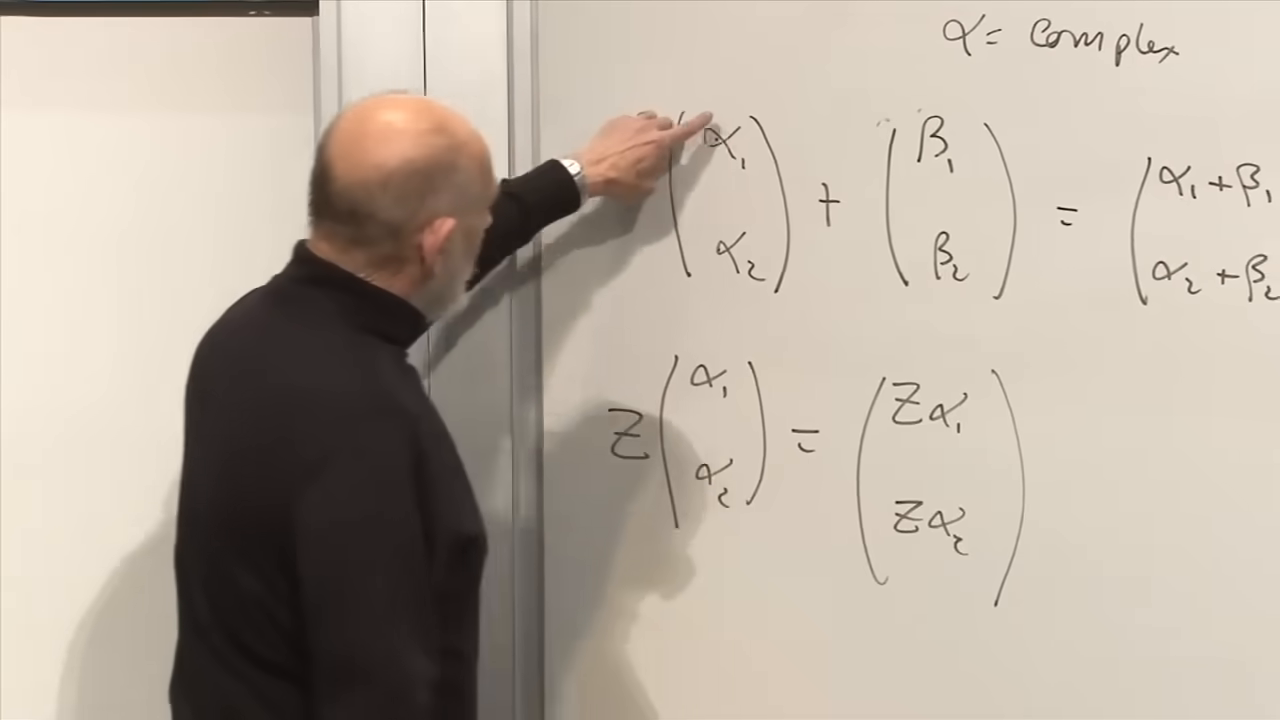
\includegraphics[width=0.88\textwidth]{lecture_01_figure_05.png}
  \caption{Les règles composante par composante pour additionner deux colonnes complexes et multiplier une colonne par un scalaire complexe.}
  \lectureframe{01:14:28}
\end{figure}

Le vecteur nul est
\begin{equation}
  \ket{0}
  =
  \begin{pmatrix}
    0\\
    0
  \end{pmatrix},
  \qquad
  \ket{\alpha}+\ket{0}=\ket{\alpha}.
\end{equation}
Les colonnes de longueur trois forment un autre espace vectoriel, et il en va de même pour toute longueur fixée. Une colonne à deux composantes ne peut pas être additionnée à une colonne à trois composantes : elles appartiennent à des espaces différents, et aucune règle composante par composante ne les relie.

\begin{classroomqa}
\audiencequestion{Un vecteur colonne est-il une matrice ?}
\lecturerresponse{Au sens général, c’est une matrice à une seule colonne. Dans ce cours, le mot \emph{matrice} désignera généralement un tableau carré, tandis qu’un tableau à une seule colonne sera appelé vecteur colonne. La distinction est terminologique ; elle ne traduit aucun désaccord sur l’algèbre.}
\end{classroomqa}

\begin{classroomqa}
\audiencequestion{L’ordre de l’addition des vecteurs a-t-il de l’importance ?}
\lecturerresponse{Non. L’addition composante par composante hérite de la commutativité des nombres complexes :
\[
  \ket{\alpha}+\ket{\beta}
  =
  \ket{\beta}+\ket{\alpha}.
\]
C’est l’un des axiomes des espaces vectoriels.}
\end{classroomqa}

\section{Vecteurs duaux : bras et kets}

À tout ket \(\ket{A}\) correspond un vecteur dans l’espace dual, noté \(\bra{A}\). L’application du ket au bra est additive, mais conjugue les scalaires complexes :
\begin{align}
  \ket{A}+\ket{B}
  &\longleftrightarrow
  \bra{A}+\bra{B},\\
  z\ket{A}
  &\longleftrightarrow
  z^*\bra{A}.
  \label{eq:qml1-antilinear-dual}
\end{align}
Cette seconde règle est la caractéristique essentielle du cas complexe. Le dual d’un multiple scalaire est multiplié par le scalaire complexe conjugué.

\begin{figure}[htbp]
  \centering
  \includegraphics[width=0.86\textwidth]{lecture_01_figure_06.png}
  \caption{La correspondance entre ket et bra et ses deux règles : les sommes deviennent des sommes, tandis que la multiplication par un scalaire est conjuguée complexe.}
  \lectureframe{01:23:15}
\end{figure}

Pour la réalisation à deux composantes,
\begin{equation}
  \ket{\alpha}
  =
  \begin{pmatrix}
    \alpha_1\\
    \alpha_2
  \end{pmatrix}
  \qquad\Longrightarrow\qquad
  \bra{\alpha}
  =
  \begin{pmatrix}
    \alpha_1^*&\alpha_2^*
  \end{pmatrix}.
  \label{eq:qml1-bra-from-ket}
\end{equation}
La conjugaison complexe réalise la correspondance avec le dual, et la notation en ligne distingue visuellement les deux types d’objets. L’équation~\eqref{eq:qml1-bra-from-ket} vérifie également directement l’équation~\eqref{eq:qml1-antilinear-dual}.

\section{Le produit scalaire}

Étant donnés \(\ket{\alpha}\) et \(\ket{\beta}\), associons le bra correspondant à \(\beta\) au ket \(\alpha\) :
\begin{equation}
  \braket{\beta}{\alpha}
  =
  \begin{pmatrix}
    \beta_1^*&\beta_2^*
  \end{pmatrix}
  \begin{pmatrix}
    \alpha_1\\
    \alpha_2
  \end{pmatrix}
  =
  \beta_1^*\alpha_1+\beta_2^*\alpha_2.
  \label{eq:qml1-inner-product}
\end{equation}
Le mot \emph{crochet} est littéralement formé à partir de \emph{bra} et de \emph{ket}. Il s’agit de l’analogue complexe d’un produit scalaire : on multiplie les composantes correspondantes puis on les additionne, en conjuguant celles du bra.

\begin{figure}[htbp]
  \centering
  \includegraphics[width=0.88\textwidth]{lecture_01_figure_07.png}
  \caption{Le tableau calcule le produit scalaire \(\braket{\beta}{\alpha}\) et obtient \(\beta_1^*\alpha_1+\beta_2^*\alpha_2\).}
  \lectureframe{01:31:25}
\end{figure}

En permutant les vecteurs, on obtient
\begin{equation}
  \braket{\alpha}{\beta}
  =
  \alpha_1^*\beta_1+\alpha_2^*\beta_2
  =
  \braket{\beta}{\alpha}^{*}.
  \label{eq:qml1-conjugate-symmetry}
\end{equation}
L’ordre compte donc en général, mais la différence se réduit à une conjugaison complexe.

\begin{classroomqa}
\audiencequestion{Peut-on définir un produit de vecteurs complexes sans conjuguer l’un des deux facteurs ?}
\lecturerresponse{On peut inventer une telle expression bilinéaire, mais le produit d’un vecteur par lui-même n’est alors pas nécessairement réel ni positif. Cette structure n’est pas adaptée à la mécanique quantique. Le produit scalaire conjugué, ou hermitien, fournit la norme et la structure probabiliste dont nous aurons besoin.}
\end{classroomqa}

\subsection{Norme et positivité}

Posons \(\beta=\alpha\) dans l’équation~\eqref{eq:qml1-inner-product} :
\begin{equation}
  \braket{\alpha}{\alpha}
  =
  \alpha_1^*\alpha_1+\alpha_2^*\alpha_2
  =
  |\alpha_1|^2+|\alpha_2|^2.
  \label{eq:qml1-norm-square}
\end{equation}
Ce nombre est égal à son propre conjugué complexe ; il est donc réel. Il est positif ou nul, et ne s’annule que pour le vecteur nul. La longueur est définie par
\begin{equation}
  \|\alpha\|
  =
  \sqrt{\braket{\alpha}{\alpha}}.
\end{equation}
Les composantes complexes donnent ainsi une longueur ordinaire, réelle et positive ou nulle.

\begin{figure}[htbp]
  \centering
  \includegraphics[width=0.88\textwidth]{lecture_01_figure_08.png}
  \caption{Le produit scalaire d’un vecteur avec lui-même au tableau : \(\braket{\alpha}{\alpha}=|\alpha_1|^2+|\alpha_2|^2\), le carré de la norme.}
  \lectureframe{01:34:40}
\end{figure}

\section{Orthogonalité et dimension}

Deux vecteurs sont orthogonaux lorsque leur produit scalaire s’annule :
\begin{equation}
  \braket{\beta}{\alpha}=0.
  \label{eq:qml1-orthogonality}
\end{equation}
La symétrie hermitienne rend cette relation indépendante de l’ordre :
\begin{equation}
  \braket{\beta}{\alpha}=0
  \quad\Longrightarrow\quad
  \braket{\alpha}{\beta}
  =
  \braket{\beta}{\alpha}^{*}
  =0.
\end{equation}

Dans l’espace à deux composantes, la paire orthogonale la plus simple est
\begin{equation}
  \ket{e_1}
  =
  \begin{pmatrix}
    1\\
    0
  \end{pmatrix},
  \qquad
  \ket{e_2}
  =
  \begin{pmatrix}
    0\\
    1
  \end{pmatrix},
  \qquad
  \braket{e_1}{e_2}=0.
  \label{eq:qml1-standard-basis}
\end{equation}

\begin{figure}[htbp]
  \centering
  \includegraphics[width=0.88\textwidth]{lecture_01_figure_09.png}
  \caption{Le tableau construit les colonnes orthogonales usuelles \((1,0)^{\mathsf T}\) et \((0,1)^{\mathsf T}\).}
  \lectureframe{01:39:50}
\end{figure}

La dimension peut se caractériser comme le nombre maximal de vecteurs non nuls mutuellement orthogonaux. Dans un espace à deux dimensions, on peut en avoir deux, mais pas trois. Pour le voir concrètement, soit
\begin{equation}
  \ket{v}
  =
  \begin{pmatrix}
    v_1\\
    v_2
  \end{pmatrix}
\end{equation}
un vecteur orthogonal aux deux vecteurs de l’équation~\eqref{eq:qml1-standard-basis}. On a alors
\begin{equation}
  \braket{e_1}{v}=v_1=0,
  \qquad
  \braket{e_2}{v}=v_2=0,
\end{equation}
et donc \(\ket{v}=\ket{0}\). Il n’existe pas de troisième vecteur non nul orthogonal aux deux autres.

\begin{classroomqa}
\audiencequestion{Le vecteur nul n’est-il pas orthogonal à tous les vecteurs, ce qui en ferait un vecteur supplémentaire ?}
\lecturerresponse{Si, d’où la nécessité de préciser que les vecteurs mutuellement orthogonaux doivent être \emph{non nuls}. Le vecteur nul n’indique aucune direction indépendante ; on l’exclut donc du décompte de la dimension.}
\end{classroomqa}

\begin{remark}Dans la représentation en colonnes, la dimension est égale au nombre de composantes. La définition par l’orthogonalité est plus abstraite et ne suppose pas qu’on ait déjà choisi des coordonnées.
\end{remark}

\section{Autres questions au tableau}

\begin{classroomqa}
\audiencequestion{La même structure vaut-elle pour un espace vectoriel de fonctions ?}
\lecturerresponse{Oui. On peut considérer une fonction comme une colonne dont les composantes \(\psi(x)\) sont indexées par une variable continue. L’addition et la multiplication par un scalaire s’effectuent point par point. Le produit scalaire correspondant prendra la forme d’une intégrale plutôt que d’une somme finie ; cette construction sera développée plus tard.}
\end{classroomqa}

\begin{classroomqa}
\audiencequestion{La multiplication d’un ket par un bra produit-elle une matrice ?}
\lecturerresponse{Oui. Le produit scalaire \(\bra{\beta}\ket{\alpha}\) contracte une ligne avec une colonne et donne un nombre. En inversant l’ordre, \(\ket{\alpha}\bra{\beta}\), on obtient un produit extérieur, c’est-à-dire une matrice carrée. Les produits scalaire et extérieur joueront tous deux un rôle important.}
\end{classroomqa}

\begin{classroomqa}
\audiencequestion{La mesure affecte-t-elle réellement le qubit, au lieu de simplement le révéler ?}
\lecturerresponse{Oui. La première mesure selon un nouvel axe prépare un nouvel état ; c’est pourquoi la répéter confirme la réponse, tandis que le retour à l’ancien axe rétablit l’incertitude. Cette perturbation inévitable distingue l’expérience quantique d’une mesure classique idéalisée, que l’on peut en principe effectuer avec une douceur arbitrairement grande.}
\end{classroomqa}

\section{Les deux volets de la construction}

Nous avons maintenant deux volets qui n’ont pas encore été réunis. Le volet expérimental indique que :
\begin{enumerate}
  \item une mesure idéale d’un qubit n’a que les issues \(\pm1\) ;
  \item la répétition immédiate de la même mesure confirme le résultat ;
  \item un changement de l’axe du détecteur modifie l’état préparé par la mesure ;
  \item pour un ensemble préparé, un analyseur incliné d’un angle \(\theta\) donne une moyenne égale à \(\cos\theta\).
\end{enumerate}
Le volet mathématique indique que :
\begin{enumerate}
  \item les états quantiques seront représentés par des vecteurs plutôt que par des points classiques ;
  \item les vecteurs pertinents forment un espace vectoriel complexe ;
  \item aux kets sont associés des bras duaux, et les bras dépendent de façon antilinéaire de la multiplication par un scalaire complexe ;
  \item le produit scalaire hermitien définit la longueur, l’orthogonalité et la dimension.
\end{enumerate}

La tâche suivante consiste à relier ces deux moitiés. L’espace d’états complexe à deux dimensions d’un qubit doit reproduire la répétabilité, le caractère aléatoire et les statistiques dépendant de l’angle de l’expérience de l’analyseur. C’est dans ce lien, et non dans une quelconque représentation classique cachée, que commence la mécanique quantique.
